\documentclass[12pt,onecolumn,a4paper,portrait]{article}
%preamble

%\usepackage{fullpage}
\usepackage{blindtext}


\usepackage{graphicx}
\usepackage{amsmath}
\usepackage{enumitem}


















\begin{document}
\section{Introduction}
\blinetext
\subsection{Sub intro}
\begin{figure*}[!ht]

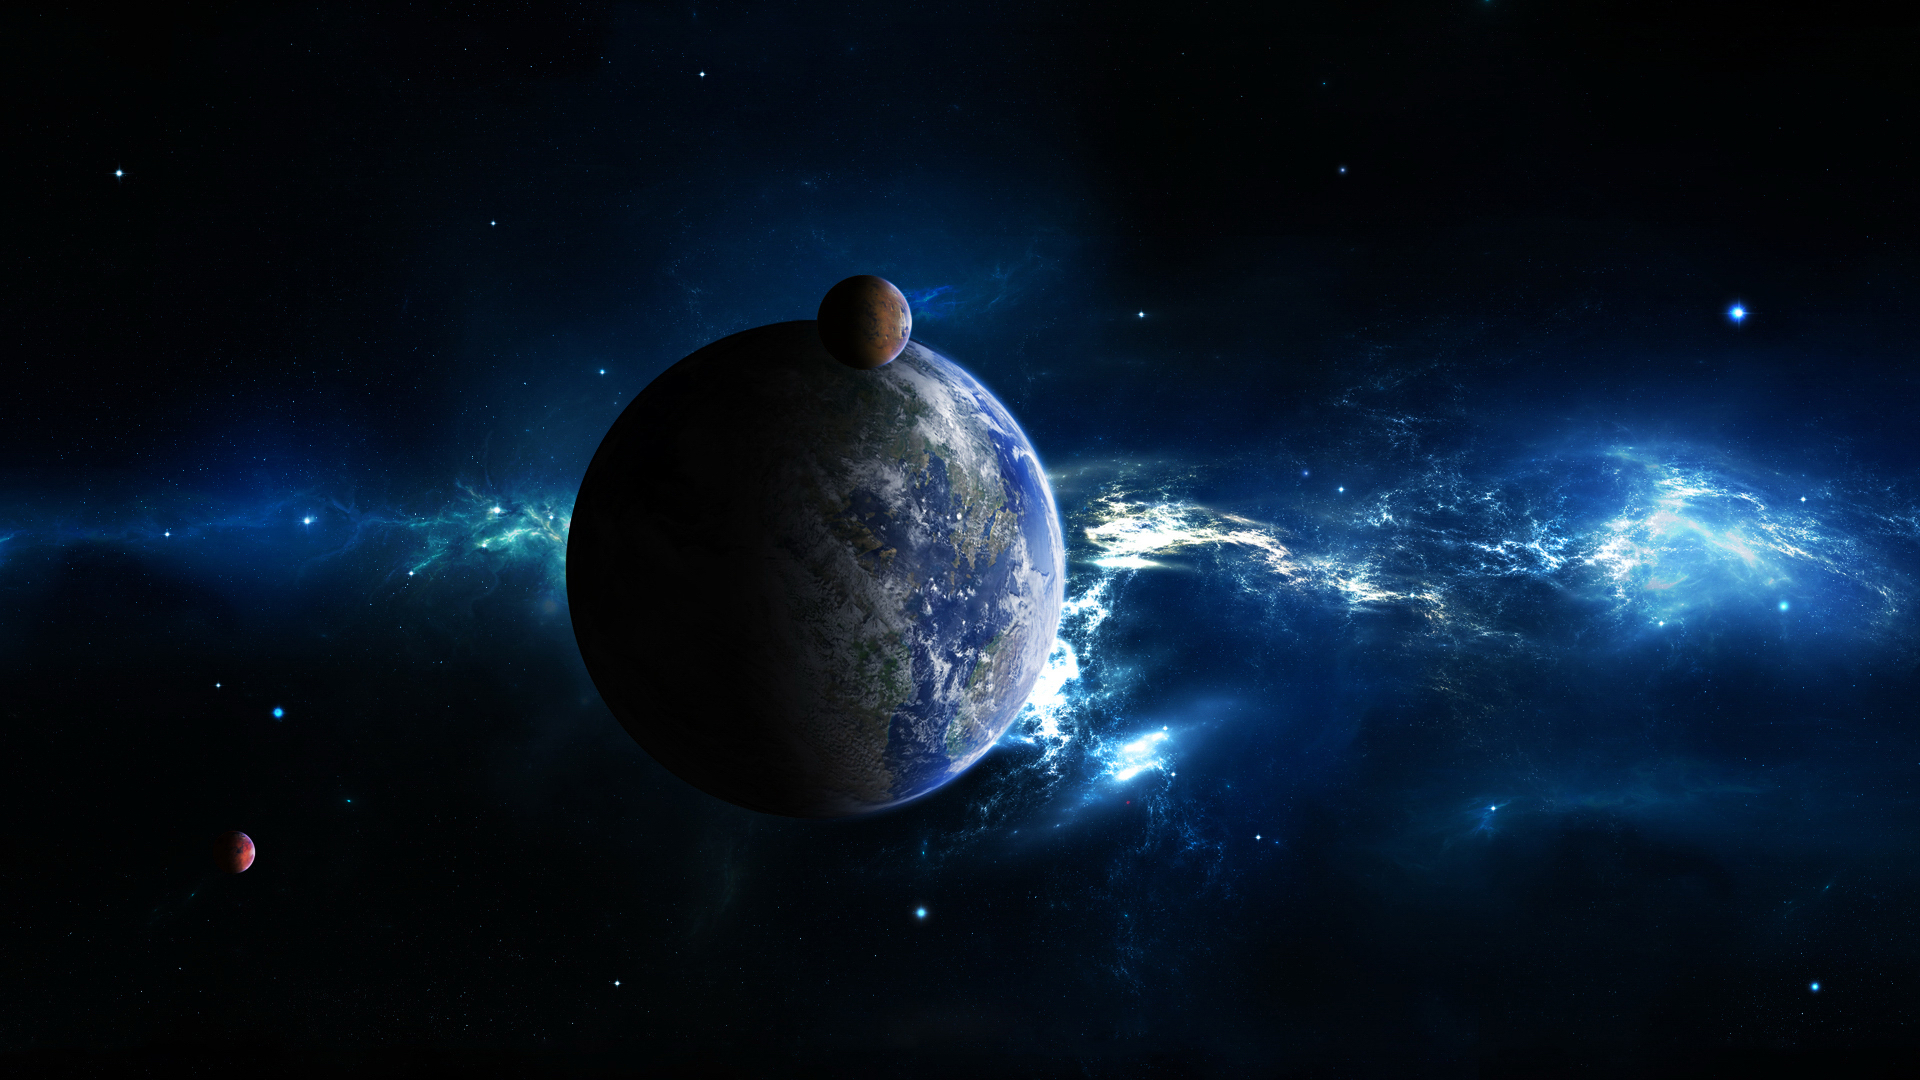
\includegraphics[width=\linewidth,height=5cm]{./images/1.jpg}
\caption{My first figure caption\label{fig:1}}
\end{figure*}


\begin{figure}[!bp]


\includegraphics[width=\linewidth]{./images/2.jpg}
\caption{My second figure caption\label{fig:2}}
\end{figure}



\tiny{tiny}\\
\small{small}\\
\footnotesize{fnsize}\\
normal\\
\large{large}\\
\Large{Large}
\\\huge{huge}\\

``\textit{italic text \emph{enphasised text}} \textbf{bold}\rq\rq{} \textsf{sans serif} \textrm{roman}



\lq{}quote\rq{}\\

`backtick\rq{}\\




\emph{enphasised text}





\blindtext
%! force our choice
%h here
%t top
%b bottom
%p page


% multicolumn and multirow package
\begin{table}[!t]

\centering

\begin{tabular}{|p{.3\linewidth}|p{.3\linewidth}|p{.2\linewidth}|}
\hline
here some random text & just some extra text& $A=B$\\
\hline
here some random text here some random texthere some random texthere some random texthere some random text& just some extra text& $A=B$\\
random text &  extra text& $B$\\
here some random text & just some extra text& $A=B$\\
random text &  extra text& $B$\\
here some random text & just some extra text& $A=B$\\
random text &  extra text& $B$\\
here some random text & just some extra text& $A=B$\\
random text &  extra text& $B$\\
\hline 
\end{tabular}
\caption{test table \label{tab:1}}

\end{table}

\blindtext





\begin{itemize}
\item A
\item B
\item C
\end{itemize}


\begin{enumerate}
\item A
\item B
\item C
\end{enumerate}


\begin{description}
\item[A] full discription
\item[B] B full disc
\item[C] Full discription
\end{description}


test-end
test--end
test---end
$test-end$
\begin{align}
E=&mc^2\\E=&\vec{b}\nonumber
\end{align}





\begin{equation}
\int_{i=0}^\infty a= A
\end{equation}



\begin{equation}
\overrightarrow{AB} \times \vec{BC} \in 
\end{equation}


$$k_{\|\|}$$
%
%\begin{equation}
%a=b \label{eqn:1}
%\end{equation}







In line math $a=b$ end line \$

\ref{eqn:2}

%
%
%\section{temp}
%\section{temp2}
%
%\section{Introduction to \LaTeX}\label{sec:intro}
%
%
%
%In section \ref{sec:2}, we have discussed some thing
%
%START\ \  \ \ \ \ \ \                   ipsum dolor sit amet, consectetuer adipiscing elit line end. 
%
%\section{temp}
%\section{temp2}
%
%\section{test chapter}\label{sec:2}
%
%
%In Intro section \ref{sec:intro}
%
%\textbackslash
%\%
%\&%alignment
%\ % space
%\\% for linebreak
%
%
%
%
%
%
%\par facilisis sem. Nullam nec mi et neque pharetra sollicitudin. Praesent imperdietmi nec ante. Donec ullamcorper, felis non sodales commodo, lectus velit ultrices augue, a dignissim nibh lectus placerat pede. Vivamus nunc nunc, molestieut, ultricies vel, semper in, velit. Ut porttitor. \par Praesent in sapien. Lorem ipsum dolor sit amet, consectetuer adipiscing elit. Duis fringilla tristique neque. Sed interdum libero ut metus.%
%
% 
%  
%  
%  
%  
%   
%    
%\noindent      Pellentesque placerat. Nam rutrum augue aleo. Morbi sed elit sit amet ante lobortis sollicitudin. Praesent blandit blanditmauris. Praesent lectus tellus, aliquet aliquam, luctus a, egestas a, turpis. PARAGRAPH CHANGE\\ Mauris lacinia lorem sit amet ipsum. Nunc quis urna dictum turpis accumsan
%END.


\end{document}

